%\documentclass[mathserif,xcolor=dvipsnames]{beamer}
\documentclass[xcolor=dvipsnames]{beamer}

%\usefonttheme{serif}
%\setbeamerfont{structure}{family=\sffamily,shape=\upshape} 

\usefonttheme{professionalfonts}

\usepackage{math}
\usepackage{util}
\usepackage{ufont}

\usetheme{Madrid}
\usecolortheme[named=MidnightBlue]{structure} 
\useoutertheme{umbcfootline} 
\setbeamertemplate{items}[ball] 
\setbeamertemplate{blocks}[rounded][shadow=true] 
\setbeamertemplate{navigation symbols}{} 

\setlength{\parskip}{1em}

\newcommand*{\as}{A}
\newcommand*{\xs}{\mathcal{X}}
\newcommand*{\ms}{\mathcal{M}}
\newcommand*{\emp}{\mathrm{emp}}



%\title[The Geometry of DBNs]{The (Real) Geometry of \\the Restricted Boltzmann Machine}
\title{Algebraic Methods for Log-Linear Models}
\author{Aaron Pribadi}
\institute[HMC]{Harvey Mudd College \\ Presentation Days}
\date{April 30, 2012}

\begin{document}

\begin{frame}[plain]
    \maketitle
\end{frame}


\begin{frame}[fragile]{Binary Data}

    \lspace
    \lspace
    \begin{columns}

    \begin{column}{0.42\textwidth}
        The votes of 232 members of the U.S. House of Representatives on
        16 selected bills.  
        
        Data are from the UCI Machine Learning Repository.
    \end{column}

    \begin{column}{0.58\textwidth}
    \begin{center}
    \begin{verbatim}
1) n y y n y y n n n n n n y y y y
2) n y n y y y n n n n n y y y n y
3) y y y n n n y y y n y n n n y y
4) y y y n n n y y y n n n n n y y
5) y n y n n n y y y y n n n n y y
    \end{verbatim}
    and 227 more \ldots
    \end{center}
    \end{column}

    \end{columns}
        
    \lspace
    {\footnotesize
    \texttt{http://archive.ics.uci.edu/ml/datasets/Congressional+Voting+Records}
    }

\end{frame}

\begin{frame}[fragile]{Binary Data}

    \lspace
    \lspace
    \begin{columns}

    \begin{column}{0.42\textwidth}
        The votes of 232 members of the U.S. House of Representatives on
        16 selected bills.  
        
        Data are from the UCI Machine Learning Repository.
    \end{column}

    \begin{column}{0.58\textwidth}
    \begin{center}
    \begin{verbatim}
1) 0 1 1 0 1 1 0 0 0 0 0 0 1 1 1 1
2) 0 1 0 1 1 1 0 0 0 0 0 1 1 1 0 1
3) 1 1 1 0 0 0 1 1 1 0 1 0 0 0 1 1
4) 1 1 1 0 0 0 1 1 1 0 0 0 0 0 1 1
5) 1 0 1 0 0 0 1 1 1 1 0 0 0 0 1 1
    \end{verbatim}
    and 227 more \ldots
    \end{center}
    \end{column}

    \end{columns}
        
    \lspace
    {\footnotesize
    \texttt{http://archive.ics.uci.edu/ml/datasets/Congressional+Voting+Records}
    }

\end{frame}

\begin{frame}{Binary Data}
    We can ask many questions about the data.
    \begin{itemize}
    \item How likely is a person to vote \texttt{0101010101010101}?
    \item If someone votes \texttt{010101010101010\_} on the first 15
    bills, what is she more likely to vote on the 16th?
    \item How do votes on the first and second bills interact?
    \item et cetera
    \end{itemize}
\end{frame}

\begin{frame}{Binary Data}
    Assume i.i.d. random variables
    \[
        X_1, X_2, \ldots, X_{232}
    \]
    with $X_i$ taking values in $\{0, 1\}^{16}$ and $X_i \sim p$.

    What is the underlying distribution $p$?
\end{frame}

\begin{frame}{Empirical Estimate}
    The obvious estimate of $p$ is
    \[
        p_\emp(x) = 
        \frac{
            \text{number of $i$ for which $X_i = x$}
        }{
            \text{number of samples}
        }.
    \]
\end{frame}

\begin{frame}{Empirical Estimate}
    The estimate of the conditional probability is 
    \[
        P[ x_{16} = 1 \mid x_1 \cdots x_{15} = 01\cdots010]
        \approx
        \frac{ \sum p_\emp(y) }{ \sum p_\emp(z) }
    \]
    where 
    \nlspace
    \begin{itemize}\nospace
    \item $y$ ranges over values where $y_1\cdots y_{15} = 01\cdots010$ and $y_{16} = 1$, and
    \item $z$ ranges over values where $z_1\cdots z_{15} = 01\cdots010$.
    \end{itemize}

    Divide by zero!
\end{frame}

\begin{frame}{Empirical Estimate}
    With sample space $\xs = \{0, 1\}^{16}$, there are $2^{16} = 65536$
    different outcomes.

    But we only have $232$ samples.
\end{frame}

\begin{frame}{The Space of Distributions}
    A probability distribution $p$ is a function $p : \xs \to \R$ such that
    \[
        \sum_{x \in \xs} p(x) = 1
        \qquad\text{and}\qquad
        p(x) \ge 0 \quad\text{for all $x \in \xs$}.
    \]
\end{frame}

\begin{frame}{The Space of Distributions}
    \lspace
    The $(n-1)$-dimensional \textbf{standard simplex} is the subset
    \[
        \Delta_{n-1} = \cdel*{ (p_1, \ldots, p_n) \in \R^{n} \:: \sum_k p_k= 1, p_k \ge 0 }
    \]
    of $\R^n$.  The points of the simplex correspond one-to-one with probability
    distributions on $n$ outcomes.
    \nlspace
    \begin{figure}\centering
        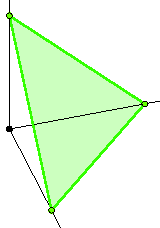
\includegraphics[width=0.2\textwidth]{2-simplex.pdf} 
        \caption{The 2-simplex}
    \end{figure}
\end{frame}

\begin{frame}{The $p \gg N$ Problem}
    When the sample space $\xs$ is large
    \[
        \dim\pdel*{\Delta_{|\xs| - 1}} = |\xs| - 1 \gg \text{number of samples}.
    \]

    This type of situation is known as `$p \gg N$'.
\end{frame}

\begin{frame}{Statistical Models}
    A \textbf{statistical model} is a subset $\ms \subset \Delta$ of the
    simplex.

    We assume that the true distribution $p$ is in this small subset.
\end{frame}

\begin{frame}{Statistical Models}
    \begin{example}[Independence]
        The \textbf{independence model} $\ms$ on the sample space $\xs = \{0,
        1\}^m$ contains distributions that factor as
        \[
            p(x) = p_1(x) \cdots p_m(x)
            \qquad\text{where}\qquad
            p_k(x) = \sum_{y_k = x_k} p(y).
        \]
        \nlspace
        \begin{itemize}
        \item For the simplex, $\dim(\Delta) = 2^m - 1$.
        \item For the model, $\dim(\ms) = m$.
        \end{itemize}
    \end{example}
\end{frame}

\begin{frame}{Log-Linear Models}
    A \textbf{log-linear model} is of the form
    \[
        \ms = \cdel[\big]{ p \in \Delta
        \::\: \log p  = (\log p_1, \ldots, \log p_n) \in V}
    \]
    where $V$ is a linear (or affine) subspace of $L(\xs)$.

    It is the discrete version of an exponential family. \\
    The log-probabilities are in a linear space.
\end{frame}

\begin{frame}{Log-Linear Models}
    \begin{example}[Independence]
    The independence model can be written as 
    \[
        \ms = \cdel[\big]{ p \in \Delta_{N-1}
        \:: \log p  \in \mathrm{rowspace}(\as)}
    \]
    where (in the case $\xs = \{0, 1\}^2$)
    \[
        \as = \kbordermatrix{
            & 00 & 01 & 10 & 11 \\
            &  1 & 1  & 0  & 0 \\
            &  0 & 0  & 1  & 1 \\
            &  1 & 0  & 1  & 0 \\
            &  0 & 1  & 0  & 1
        }.
        \qquad
        \text{\footnotesize (not full rank)}
    \]
    \end{example}
\end{frame}

\begin{frame}{A Bet on Sparsity}
    We can think of this as an approximation by a basis expansion. 

    With functions $f_i$ for $i \in I$, approximate
    \[
        \log p_\emp \approx \sum_{i \in I} \lambda_i f_i
    \]
    where most $\lambda_i$ are zero.

    ($\mathrm{span}\{f_i \:: \lambda_i \ne 0\}$ corresponds to a low-dimensional log-linear
    model.)
\end{frame}

\begin{frame}{A Bet on Sparsity}
    A \textbf{sparse approximation} has `a lot of zeros'. 
    
    Hastie et al. in \emph{The Elements of Statistical Learning} (2009):
    \begin{quote}
        Use a procedure that does well in sparse problems, since no procedure
        does well in dense problems.
    \end{quote}
\end{frame}

\begin{frame}{Log-Linear Lasso}
    \lspace
    Buchman et al.* outline a procedure for finding sparse models.

    Let $\{f_1, \ldots, f_m\}$ be a spanning set for $L(\xs)$.  Minimize
    \[
        -\sum_{j=1}^N \pdel*{\sum_{i=1}^m \beta_i f_i(z_j)}
        + \lambda \sum_{i=1}^m |\beta_i|
    \]
    for data $\{z_1, \ldots, z_N\}$ and hyperparameter $\lambda > 0$.

    \lspace
    {\footnotesize
        ($*$) ``On sparse, spectral and other parametrizations of binary probabilistic
        models''.  \emph{Proceedings of the 15th International Conference on
        Artificial Intelligence and Statistics}.
    }
\end{frame}

\begin{frame}{The Automorphism Group}
    There are two natural operations on $\xs = \{0, 1\}^m$:
    \begin{itemize}
    \item flipping a bit, and
    \item rearranging the bits.
    \end{itemize}

    These generate the \textbf{hyperoctahedral group} $S_2 \wr S_m$,  \\
    which is the automorphism group of $\xs$.
\end{frame}

\begin{frame}{The Automorphism Group}
    You can think of it as the automorphism group of the hypercube graph.
    \begin{figure}[h]
        \centering
        % http://code.google.com/p/graph-theory-algorithms-book/
        % GPL Documentation Licence

        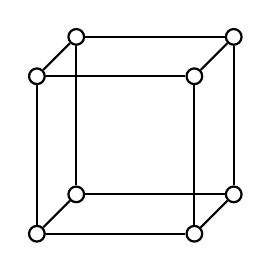
\begin{tikzpicture}
        [nodedecorate/.style={shape=circle,inner sep=2pt,draw,thick},%
          linedecorate/.style={-,thick}]
        %% nodes or vertices
        \foreach \nodename/\x/\y in {1/0/0, 2/2/0, 3/2/2, 4/0/2, 5/0.5/0.5,
          6/2.5/0.5, 7/2.5/2.5, 8/0.5/2.5}
        {
          \node (\nodename) at (\x,\y) [nodedecorate] {};
        }
        %% edges or lines
        \path
        \foreach \startnode/\endnode in {1/2, 2/3, 3/4, 4/1, 5/6, 6/7, 7/8,
          8/5, 1/5, 2/6, 3/7, 4/8}
        {
          (\startnode) edge[linedecorate] node {} (\endnode)
        };
        \end{tikzpicture}

        \caption{The $3$-hypercube graph}
        \label{fig:hypercube}
    \end{figure}
\end{frame}

\begin{frame}{An Invariance Principle}
    If a subspace $V \subset L(\xs)$ is `important' across many different data sets
    on $\xs$, then $V$ should be invariant under the automorphism group of
    $\xs$.

    More generally, statistical procedures should respect the symmetries of
    $\xs$.
\end{frame}

\begin{frame}{The Isotypic Decomposition}
    From the representation theory of finite groups, \\
    $L(\xs)$ has an \textbf{isotypic decomposition}.
    \[
        L(\xs) = \bigoplus_{\rho \in \widehat{G}} m_\rho W_\rho
    \]
    This is the `finest' uniquely defined decomposition into invariant
    subspaces.
    
    \lspace
    {\footnotesize
        This is technically over $\mathbb C$, but it often also works over $\R$.
    }
\end{frame}

\begin{frame}{The Isotypic Decomposition}
    The isotypic decomposition of $L(\xs)$ for $\xs = \{0, 1\}^m$ is
    multiplicity free. \\
    Each component is an eigenspace of the Laplacian matrix for the hypercube.
    \[
        \kbordermatrix{
            & 00 & 01 & 10 & 11 \\
        00  &  2 & -1  & -1  & 0 \\
        01  &  -1 & 2  & 0  & -1 \\
        10  &  -1 & 0  & 2  & -1 \\
        11  &  0 & -1  & -1  & 2
        }
    \]\[
        V_0 = \adel*{\begin{rmatrix} 1 \\ 1 \\ 1 \\ 1\end{rmatrix}}
        \qquad
        V_2 = \adel*{
            \begin{rmatrix} 1 \\ -1 \\ -1 \\ 1\end{rmatrix},
            \begin{rmatrix} 1 \\ -1 \\  1 \\ -1\end{rmatrix}
            }
        \qquad
        V_4 = \adel*{\begin{rmatrix} 1 \\ -1 \\ -1 \\ 1\end{rmatrix}}
    \]
\end{frame}

\begin{frame}{Homogeneous Spaces and $K$-Invariant Vectors}
    The log-linear lasso uses a spanning set of $L(\xs)$.  

    Is there a natural choice?
\end{frame}

\begin{frame}{Homogeneous Spaces and $K$-Invariant Vectors}
    The action of $G = S_2 \wr S_m$ on $\xs = \{0, 1\}^m$ is transitive,\\
    so $\xs$ is a \textbf{homogeneous space}.

    For any $x_0 \in \xs$, we can write
    \[
        \xs \cong G / K
    \]
    where $K = \mathrm{fix}_G(x_0)$.
\end{frame}

\begin{frame}{Homogeneous Spaces and $K$-Invariant Vectors}
    Furthermore, $(G, K)$ is a \textbf{Gelfand pair} (for $\xs = \{0, 1\}^m$).

    This means that $L(\xs)$ is multiplicity-free
    \[
        L(\xs) = W_{\rho_0} \oplus \cdots \oplus W_{\rho_m}.
    \]
    and that for each irreducible/isotypic component
    \[
        \dim (W_\rho)^K = 1
    \]
    i.e. there is exactly one $K$-invariant vector up to scaling.
\end{frame}

\begin{frame}{A Natural Spanning Set for $L(\xs)$}
    Different choices of base point $x_0 \in \xs$ yield different stabilizers $K
    = \mathrm{fix}_G(x_0)$.

    I showed that in each $W_\rho$, the set of all vectors invariant under some
    stabilizer spans $W_\rho$.

    This spanning set
    \begin{itemize}
    \item depends only on $\xs$ and its automorphism group, 
    \item is invariant under the action of the automorphism group, and
    \item respects the isotypic decomposition.
    \end{itemize}
\end{frame}

\begin{frame}[fragile]{A Natural Spanning Set for $L(\xs)$}
    For $\xs = \{0, 1\}^3$, 
    {\footnotesize
    \begin{gather*}
        W_0 = \adel*{
        \begin{rmatrix}
            1 \\ 1 \\ 1 \\ 1 \\ 1 \\ 1 \\ 1 \\ 1
        \end{rmatrix}
        }
        \qquad
        W_2 = \adel*{
        \begin{rmatrix}
            3 \\ 1 \\ 1 \\ -1 \\ 1 \\ -1 \\ -1 \\ -3
        \end{rmatrix}
        ,
        \begin{rmatrix}
            1 \\ 3 \\ -1 \\ 1 \\ -1 \\ 1 \\ -3 \\ -1
        \end{rmatrix}
        ,
        \begin{rmatrix}
            1 \\ -1 \\ 3 \\ 1 \\ -1 \\ -3 \\ 1 \\ -1
        \end{rmatrix}
        ,
        \begin{rmatrix}
            1 \\ -1 \\ -1 \\ -3 \\ 3 \\ 1 \\ 1 \\ -1
        \end{rmatrix}
        } 
    \\
        W_4 = \adel*{
        \begin{rmatrix}
            3 \\ -1 \\ -1 \\ -1 \\ -1 \\ -1 \\ -1 \\ 3 
        \end{rmatrix}
        ,
        \begin{rmatrix}
            -1 \\ 3 \\ -1 \\ -1 \\ -1 \\ -1 \\ 3 \\ -1
        \end{rmatrix}
        ,
        \begin{rmatrix}
            -1 \\ -1 \\ 3 \\ -1 \\ -1 \\ 3 \\ -1 \\ -1
        \end{rmatrix}
        ,
        \begin{rmatrix}
            -1 \\ -1 \\ -1 \\ 3 \\ 3 \\ -1 \\ -1 \\ -1
        \end{rmatrix}
        }
        \qquad
        W_6 = \adel*{
        \begin{rmatrix}
            1 \\ -1 \\ -1 \\ 1 \\ -1 \\ 1 \\ 1 \\ -1
        \end{rmatrix}
        }
        \qquad
    \end{gather*}
}
\end{frame}

\begin{frame}{Interpretability}
    A subspace is important if the projection of $\log p$ into it is large.

    Using only the first three bills from our data, the empirical distribution
    is
    \begin{center}
    \begin{tabular}{l | cccc cccc}
        $x$ & 000 & 001 & 010 & 011 & 100 & 101 & 110 & 111 \\
        \hline
        $\log p(x)$ & -1.60 & -2.05 & -1.78 & -2.45 & -3.25 & -1.78 & -2.81 & -1.92
    \end{tabular}
    \end{center}
    For example, the projection onto the vector $[1, 3, -1, 1, -1, 1, -3, -1]^T$
    \\
    from $W_2$ has norm $3.41$, which is relatively large.
\end{frame}

\begin{frame}{Future Directions}
    Mixture models, and the restricted Boltzmann machine:
    \[
        p(x) \propto \exp\pdel*{-\sum_{i,j} \beta_{ij}x_i h_j - \sum_i \gamma_i
        x_i - \sum_j \delta_j h_j}
    \]
\end{frame}

\begin{frame}{End}
    \begin{center}
    Thanks!
    \end{center}
\end{frame}

\end{document}
